\documentclass{beamer}

\usepackage[utf8]{inputenc}
\usepackage[english]{babel}
\usepackage{xcolor}
\usepackage{graphicx}
\usepackage{booktabs}
\usepackage{tabularx}
\usepackage[edges]{forest}

\usetheme{Berkeley}
\usecolortheme{dolphin}

\setbeamerfont{title}{size=\huge, series=\bfseries}
\setbeamertemplate{navigation symbols}{}

\title[LLM Benchmark]{LLM Benchmark for PDDL Planning}
\subtitle{Evaluating planning and reasoning capabilities of Large Language Models}
\date{3 July 2026}

\begin{document}

\begin{frame}
    \titlepage
    \vspace{-0.4cm}
    \begin{columns}
        \begin{column}{0.5\textwidth}
            \centering
            \textbf{Students:}\\
            Simone Migliaccio\\
            Simone Spezia\\
            Alberto Varini
        \end{column}
        \begin{column}{0.5\textwidth}
            \centering
            \textbf{Professors:}\\
            Allegra De Filippo\\
            Michele Lombardi
        \end{column}
    \end{columns}
\end{frame}

\section{Introduction}

\begin{frame}{Research Question}\footnotesize
    \textcolor{blue}{\textbf{Question:}} can LLMs solve PDDL planning tasks or do they mainly generate plausible action sequences?

    \vspace{0.4cm}
    With this question in mind, we designed this modular and scalable Benchmark to evalute three aspects:
    \begin{itemize}
        \item whether a generated plan formally reaches the goal;
        \item whether the action sequence is grounded in the PDDL domain;
        \item whether iterative repair improves planning or only resamples attempts.
    \end{itemize}

    The goal is not only to rank models, but to explain how and why they succeed or fail.
\end{frame}

\section{Benchmark Structure}

\begin{frame}{Benchmark General Structure}\scriptsize
        \begin{columns}
        \begin{column}{0.5\textwidth}
            \texttt{Benchmark\_Framework} is the runnable benchmark layer. Only the core folders are shown here.
            \begin{itemize}
                \setlength{\itemsep}{2pt}
                \setlength{\parskip}{0pt}
                \setlength{\parsep}{0pt}
                \setlength{\topsep}{0pt}
                \setlength{\partopsep}{0pt}
                
                \item \textit{tasks}: selected PDDL domains and instances.
                \item \textit{prompts} and \textit{protocols}: prompt text, direct planning and repair settings.
                \item \textit{models}: backend registries and adapter configuration.
                \item \textit{runner}: suite and single-case execution logic.
                \item \textit{evaluators}: parser, VAL validation, metrics and error taxonomy.
                \item \textit{outputs}: raw, parsed and scored benchmark artifacts.
                \item \textit{reporting}: post-run plots and JSON reports.
                \item \textit{utils}: bundled VAL validator binaries.
            \end{itemize}
        \end{column}
        
        \begin{column}{0.5\textwidth}
            \begin{forest}
            for tree={
                font=\ttfamily,
                grow'=0,
                child anchor=west,
                parent anchor=south,
                anchor=west,
                calign=fixed edge angles,
                edge={draw, semithick},
                l sep = 7pt,
                s sep = 2pt,
                inner sep = 2.5pt,
                folder,
            }
            [Benchmark\_Framework/
                [evaluators/]
                [models/]
                [outputs/]
                [prompts/]
                [protocols/]
                [reporting/]
                [runner/]
                [tasks/]
                [utils/]
                [run\_benchmark.py]
            ]
            \end{forest}
        \end{column}
    \end{columns}
    
\end{frame}

\begin{frame}{Benchmark Structure}\footnotesize
    The project is organized as a reproducible pipeline:

    \vspace{0.25cm}
    \centering
    \texttt{PDDL tasks + prompts + protocols + model registries}

    \vspace{0.18cm}
    $\Downarrow$

    \vspace{0.18cm}
    \texttt{run\_benchmark.py}

    \vspace{0.18cm}
    $\Downarrow$

    \vspace{0.18cm}
    \texttt{model adapter -> parser -> VAL validator -> metrics}

    \vspace{0.18cm}
    $\Downarrow$

    \vspace{0.18cm}
    \texttt{outputs/raw + outputs/parsed + outputs/scored}

    \vspace{0.35cm}
    \raggedright
    The same task set can be evaluated across different models while keeping prompts, parsing, validation and scoring comparable.
    Also, without worring of the backend used.
\end{frame}

\section{Problem Selection}

\begin{frame}{Problem Selection}\footnotesize
    The benchmark uses a small but meaningful set of PDDL domains.

    \vspace{0.3cm}
    Domains and instances are selected using two complementary criteria:
    \begin{itemize}
        \item \textbf{difficulty:} based on grounded actions, goals, numeric features and topology;
        \item \textbf{reasoning category:} based on the dominant planning skill required by the domain.
    \end{itemize}

    \vspace{0.3cm}
    To do this, we take informations from \texttt{score\_domains\_complexity.py}.

    This makes failures easier to interpret: a model can be compared by task difficulty and by type of reasoning required.
\end{frame}

\begin{frame}{Selected PDDL Domains}\footnotesize
    By looking at the ranking of the difficulty scores, we decided that the final set composed by three reasoning categories with both hard and easy domains.

    \vspace{0.25cm}
    \begin{columns}[T]
        \begin{column}{0.48\textwidth}
            \centering
            \textbf{Hard Set}
            \begin{itemize}
                \item settlersnumeric -- numerical optimization
                \item rover -- logistics
                \item block-grouping -- spatial planning
            \end{itemize}
        \end{column}
        \begin{column}{0.48\textwidth}
            \centering
            \textbf{Easy Set}
            \begin{itemize}
                \item fo-counters -- numerical optimization
                \item expedition -- logistics
                \item fo-sailing -- spatial planning
            \end{itemize}
        \end{column}
    \end{columns}

    \vspace{0.3cm}
    Temporal planning and symbolic logic are not included in the final set because the available domain coverage was too limited.
\end{frame}

\section{Models}

\begin{frame}{Models and Execution Backends}\footnotesize
    The framework supports both local and hosted execution.

    \vspace{0.2cm}
    \begin{itemize}
        \item \textbf{Leonardo HPC:} local Hugging Face execution with direct control of the environment.
        \item \textbf{NVIDIA API:} hosted backend for recent open-weight models.
        \item \textbf{VAL:} external validator used for formal plan correctness.
    \end{itemize}

    \vspace{0.25cm}
    To decide which LLMs to use on Leonardo, we used whichLLM. This tool permits us to estimate which recent LLMs can run on the available local hardware.
\end{frame}

\begin{frame}{Model Pool}\scriptsize
    \centering
    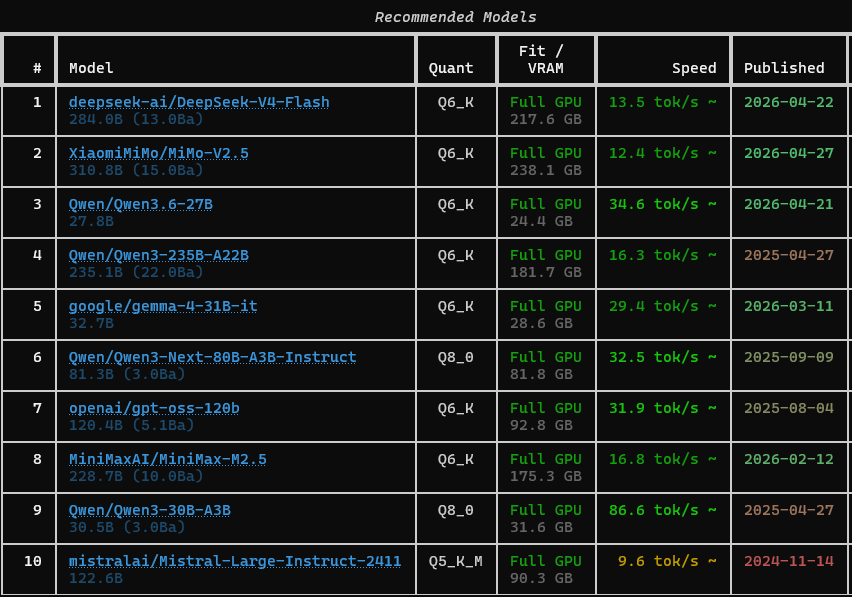
\includegraphics[width=0.92\linewidth,height=0.43\textheight,keepaspectratio]{rankLLMs.png}

    \vspace{0.18cm}
    \renewcommand{\arraystretch}{1.15}
    \begin{tabularx}{\textwidth}{l>{\raggedright\arraybackslash}X}
        \toprule
        \textbf{Backend} & \textbf{Models in the benchmark pool} \\
        \midrule
        Leonardo HPC & Gemma 4 31B IT, Phi-4, GPT-OSS 120B, Qwen 3.6 27B \\
        NVIDIA API & GPT-OSS 120B, Kimi K2.6, Llama 3.3 70B Instruct, Nemotron 3 Nano 30B A3B, Nemotron 3 Ultra 550B A55B, Phi-4 Mini Instruct, Qwen 3.5 122B A10B \\
        \bottomrule
    \end{tabularx}
\end{frame}
\section{Outputs}

\begin{frame}{Output Pipeline}\footnotesize
    Each benchmark case produces three aligned artifacts:

    \vspace{0.25cm}
    \begin{itemize}
        \item \textbf{Raw:} prompt messages, model output and provider-side reasoning text when available.
        \item \textbf{Parsed:} extracted output and reasoning PDDL actions, final plan text and formatting issues.
        \item \textbf{Scored:} VAL result, solved flag, iterations used and repair feedback.
    \end{itemize}

    \vspace{0.35cm}
    This separation keeps generation, extraction and evaluation independent, so parser errors and planning failures can be diagnosed separately.
\end{frame}

\begin{frame}{Validation and Repair Loop}\footnotesize
    VAL is the external check that decides whether the extracted plan is valid.

    \vspace{0.25cm}
    \begin{itemize}
        \item The final action sequence must be executable and must reach the goal.
        \item Prefix validation identifies where the first validity occurs.
        \item Failure types separate hallucinations, object errors and precondition failures.
        \item Iterative repair sends comprehensive feedback from previous iteration to the model for the next attempt.
    \end{itemize}

    \vspace{0.3cm}
    A case is counted as solved only when the submitted plan passes formal validation, not when a valid plan is identified in the reasoning.
\end{frame}

\section{Evaluation}

\begin{frame}{Evaluation Metrics}\footnotesize
    The metric set answers complementary questions:

    \vspace{0.2cm}
    \begin{tabularx}{\textwidth}{l>{\raggedright\arraybackslash}X}
        \toprule
        \textbf{Metric} & \textbf{Question answered} \\
        \midrule
        SR & Did the model eventually solve the task? \\
        FASR & Could it solve the task on the first attempt? \\
        IWSR / Retry Gap & Did repair help efficiently or only add retries? \\
        Executability & How much of the plan can run before the first precondition failure? \\
        Hallucination / PAS & Are failures caused by grounding or precondition reasoning? \\
        CoTaL & Does reasoning text align with the final extracted plan? \\
        PS & What is the compact planning score across signals? \\
        \bottomrule
    \end{tabularx}
\end{frame}

\section{Results}

\begin{frame}{Main Results}\footnotesize
    \centering
    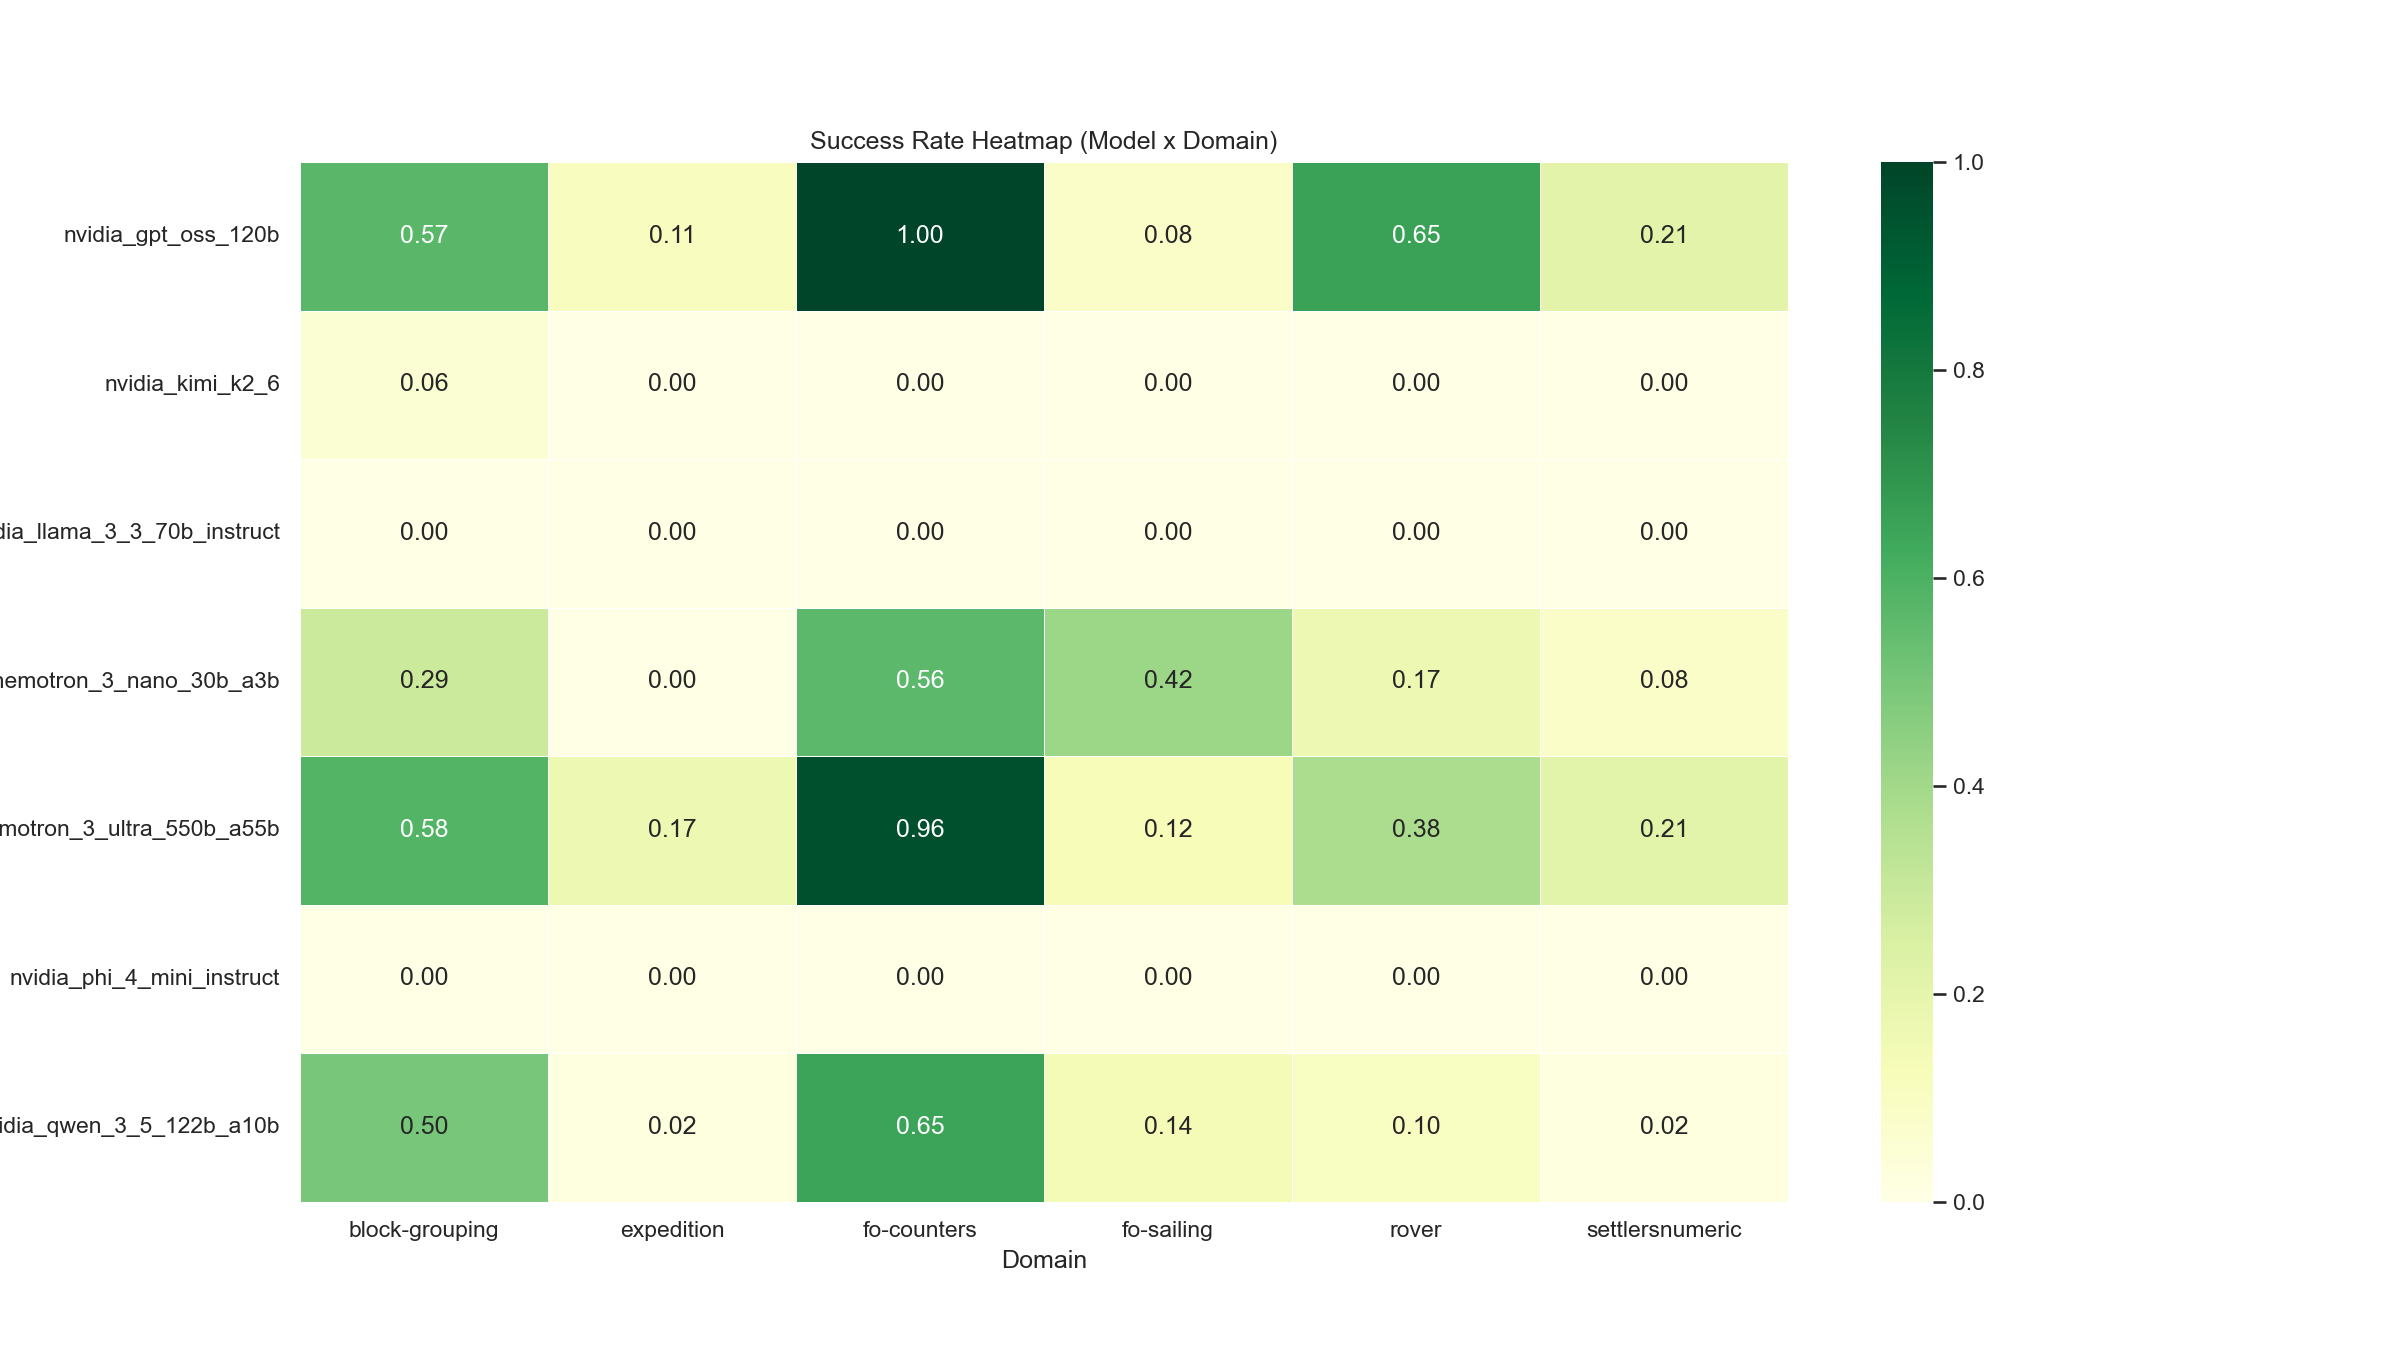
\includegraphics[width=0.95\linewidth,height=0.68\textheight,keepaspectratio]{../../results/final_evaluation_results/success_rate_heatmap.png}

    \vspace{0.2cm}
    This graph can tell us whther a model is good in finding a plan for a domain.
    By itself it cannot answer the main question, but can gives us insights on the broad capability of the models.
\end{frame}

\begin{frame}{Retries Help, But They Do Not Prove Planning}\footnotesize
    \centering
    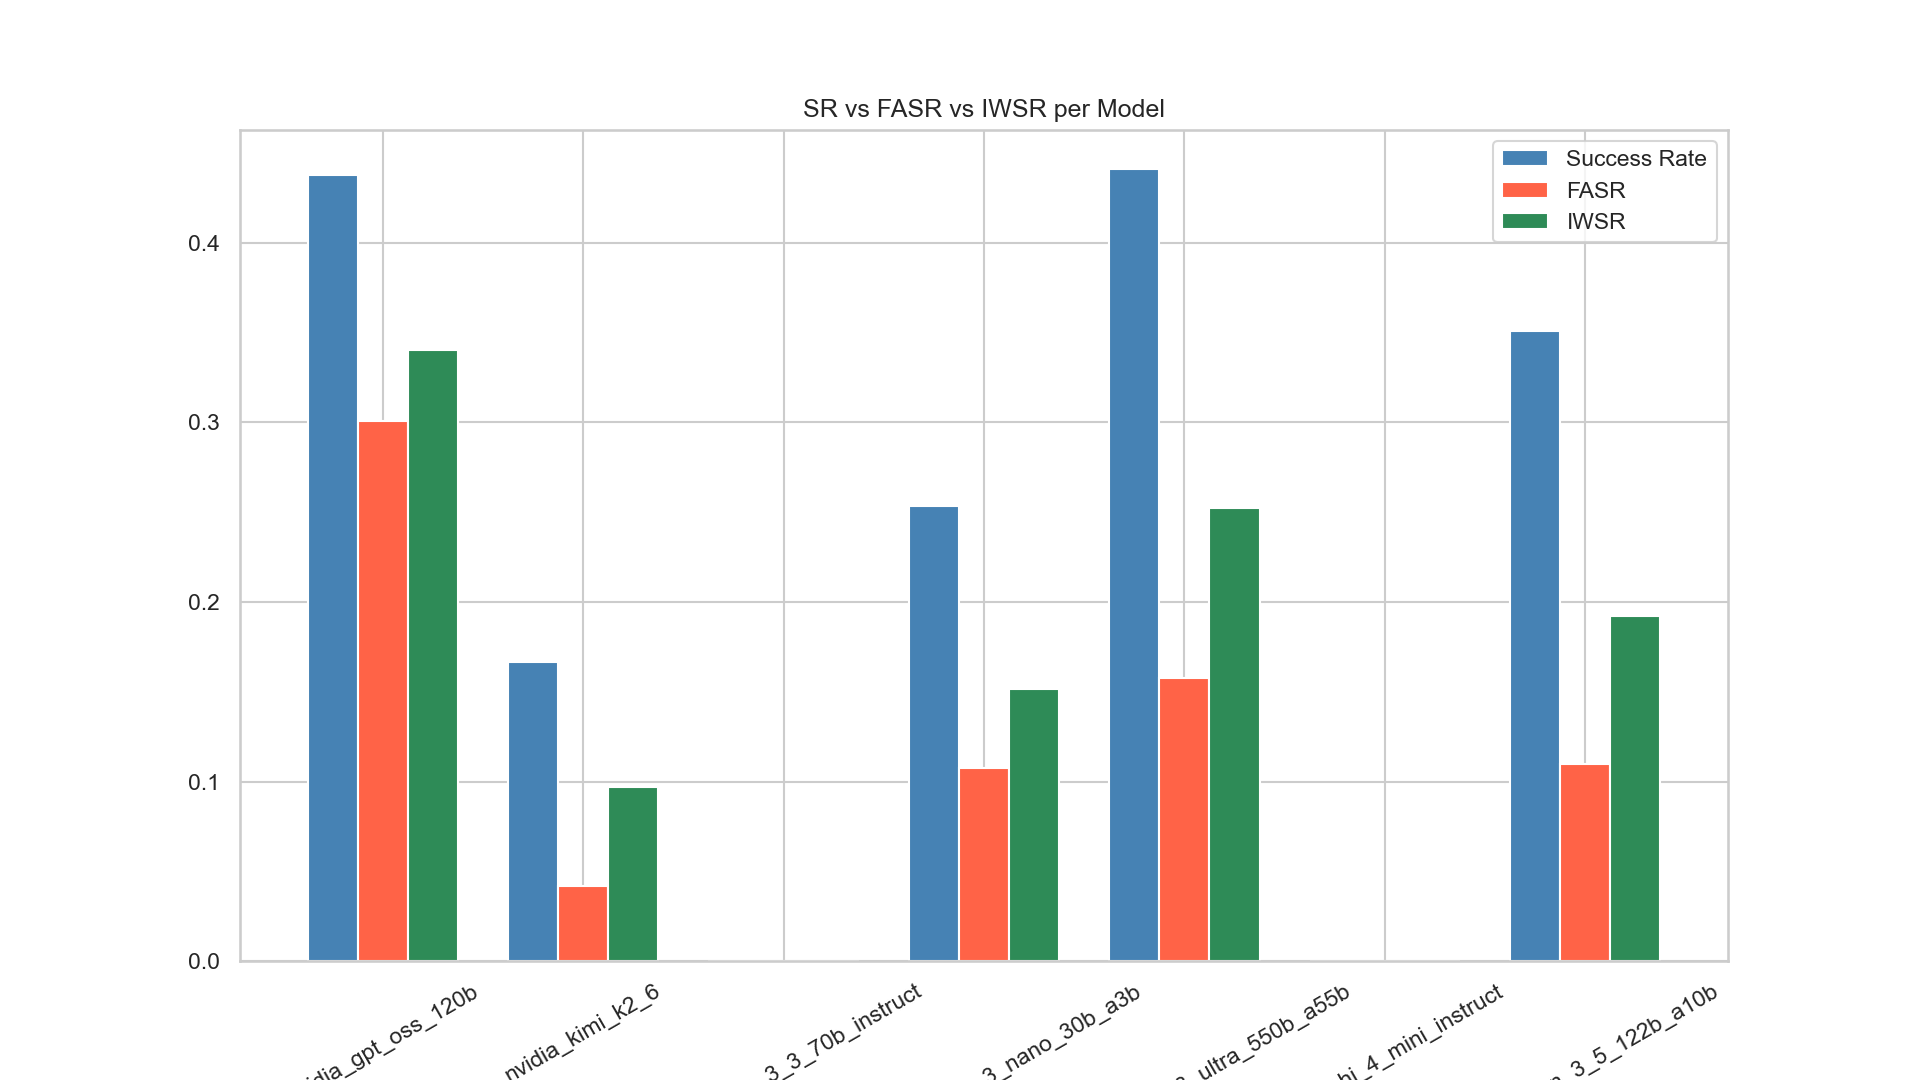
\includegraphics[width=0.95\linewidth,height=0.68\textheight,keepaspectratio]{../../results/final_evaluation_results/sr_fasr_iwsr_by_model.png}

    \vspace{0.2cm}
    By loogink at the succes rate, one would think that the iterations helps to find a velid plan.
    In reality, we need to look at the \texttt{IWSR} coloumn. This metric tells us that the iteration aren't as usefull as it seams, because the LLMs do not use fully and correctly the feedbacks.
\end{frame}

\begin{frame}{Reasoning Capabilities}\footnotesize
    \centering
    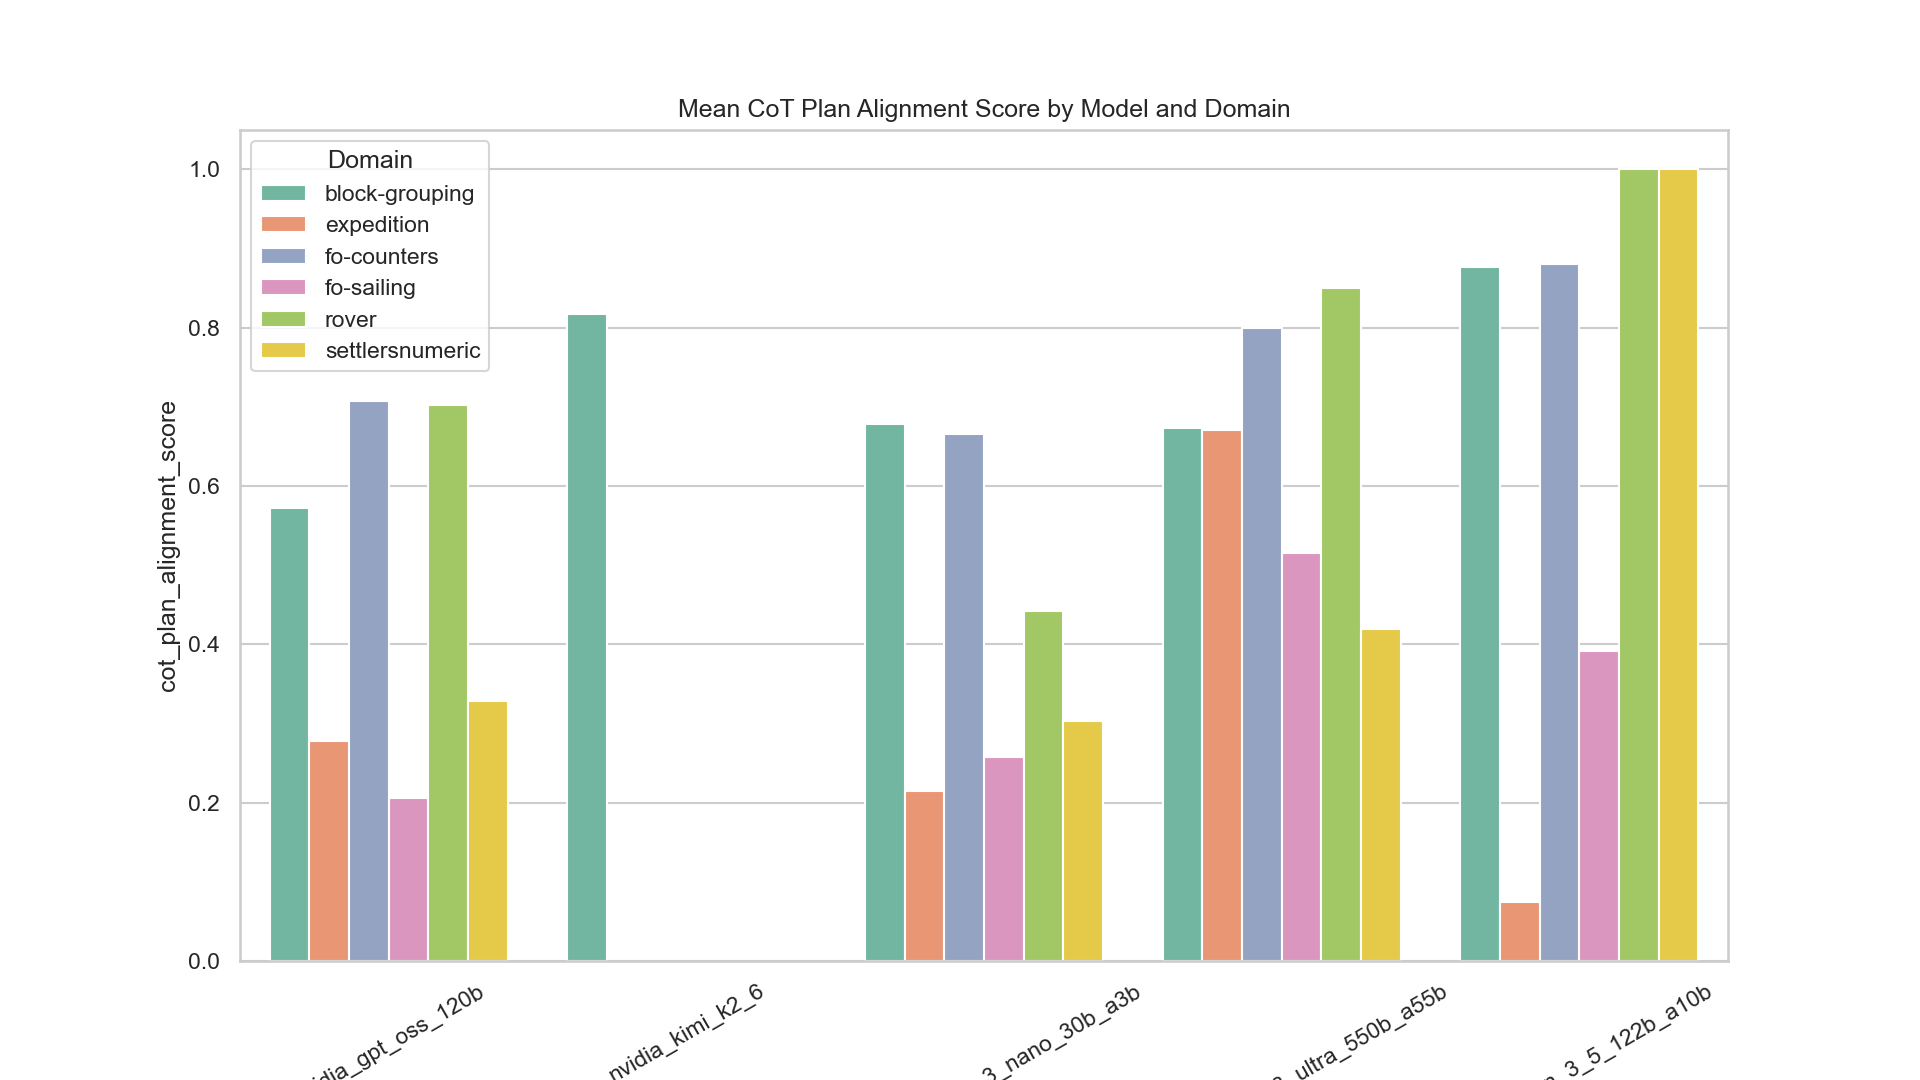
\includegraphics[width=0.95\linewidth,height=0.68\textheight,keepaspectratio]{../../results/final_evaluation_results/cot_alignment_by_model_domain.png}

    \vspace{0.2cm}
    CoTaL checks for reasoning traces in the extracted plans. Therefore, it helps assess whether LLMs maintain consistency between what they reasoned about and what they ultimately generated.
\end{frame}
\section{Conclusions}

\begin{frame}{Conclusions and Future Work}\footnotesize
    \textbf{Main conclusion:} LLMs can sometimes solve PDDL tasks, but robust long-horizon planning remains fragile.

    \vspace{0.3cm}
    \begin{itemize}
        \item The benchmark provides a reproducible pipeline from generation to formal validation.
        \item Current models often behave as repair-assisted generators rather than deterministic planners.
        \item Failures are diagnosable through executability, hallucination, PAS, retry behavior and CoTaL.
    \end{itemize}

    \vspace{0.25cm}
    \textbf{Next steps:}
    \begin{itemize}
        \item expand the domain set and model matrix;
        \item test stronger feedback strategies;
        \item deepen reasoning-trace analysis across domains and releases.
    \end{itemize}
\end{frame}

\end{document}
